\chapter{Applying the Flow Equations: 1D Bose Polaron in the Heavy Impurity Limit}\label{Results}
\section{In Combination with a Bogoliubov Transformation}
\begin{figure}[H]
    \centering
    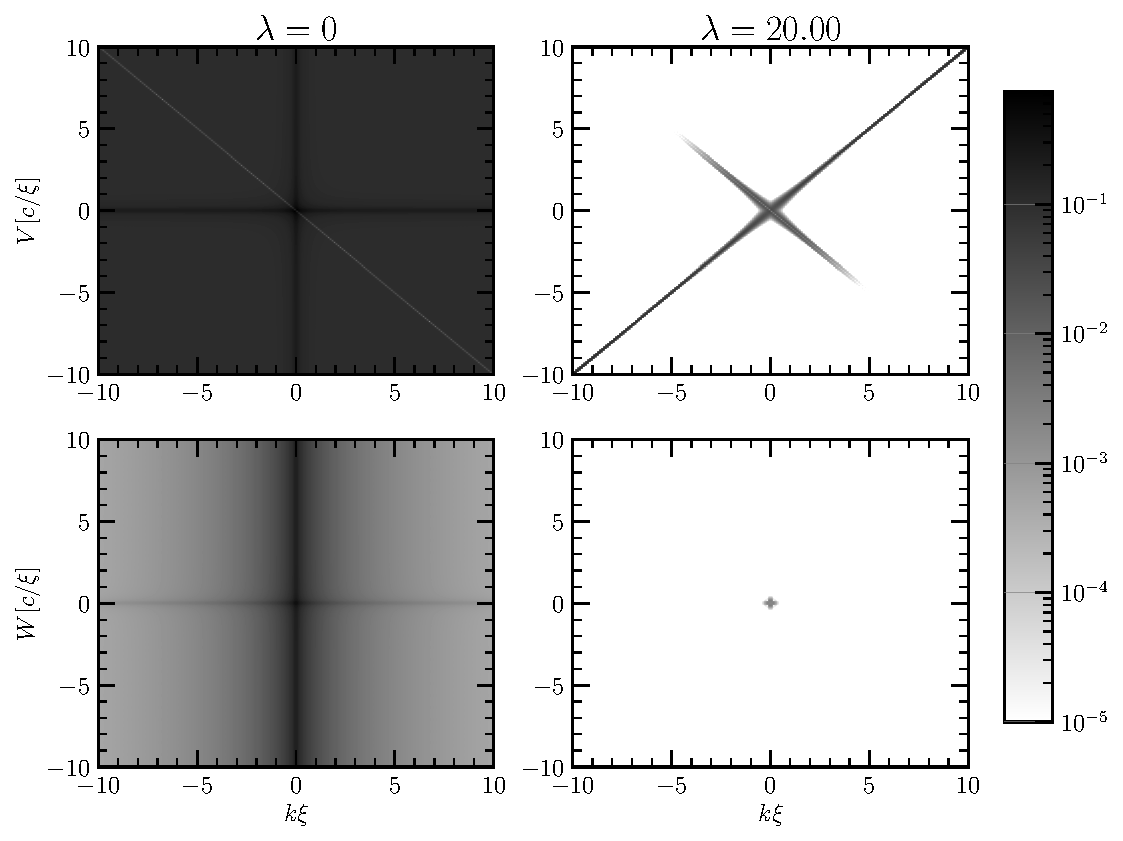
\includegraphics[width=\textwidth]{figures/plots/PDF/FlowIllustration.pdf}
    \caption[Flow Visualization for $\eta=10$]{Visualization of how the flow progresses for $\eta=10$ by shading larger absolute values for $V_{k,k^\prime},W_{k,k^\prime}$ darker. It is of note that on the ordinate and abscissa $0\widehat = \pm \lambda_{IR}\xi=\pm 0.1$. We see that good suppression occurs for all $W_{k,k^\prime}$, with slower convergence for smaller $|k|,|k^\prime|$.  Meanwhile, the matrix elements near the diagonal $V_{k,k}$ decay significantly slower than most off-diagonal elements. Also, matrix elements $V_{k,-k}$ converge, but to a value different from zero. Note that the values of $V$ near the main diagonal would  become even smaller if the flow were to progress further. This can be checked numerically by evaluating if $\mathrm{sgn}\left( V_{k,k^\prime}\right)=-\mathrm{sgn}\left( \partial_\lambda V_{k,k^\prime}\right)$ is fulfilled.}
    \label{FlowIllustration}
\end{figure}
As seen in Figure \ref{FlowIllustration}, the flow equations achieve the desired diagonalization except for terms $V_{k,-k}$. This is because $\omega_k=\omega_{-k}\forall k$ implies that the first order contribution in $\partial_\lambda V_{k,-k} =...$ vanishes. This is not a problem for the main diagonal terms $V_{k,k}$ because those have been "manually" set to zero by moving them in the diagonal part $\ham_0$ of the Hamiltonian. We can conclude that if we were not to stop the flow at a finite $\lambda$, our Hamiltonian would be approximately of the form 
\begin{equation}
\ham^\prime \defeq \Sum_{k}\left(\tilde\omega_k \CR_k\AN_k + \tilde V_{k,-k}\CR_k\AN_{-k}\right)
\end{equation}
for some $\tilde\omega_k,\tilde V_{k,k^\prime}$.\\
In principle, this could be brought into diagonal form by performing a Bogoliubov transformation for each summand by hand. But we will use the more general Bogoliubov transformation \ref{Bogoliubov Transformation Def}\footnote{For the numerics we again refer to the source code "Bogoliubov\_Transformation.py" in \url{https://github.com/SufficientlySmooth/Bachelor-Thesis-Numerics}} instead because, as can be seen in the figure \ref{FlowIllustrationInsufficient}, there are interaction strengths where not all $W_{k,k^\prime}$ vanish.
\begin{figure}[H]
    \centering
    \includegraphics[width=\textwidth]{figures/plots/PDF/FlowIllustration\_insufficient\_convergence.pdf}
    \caption[Flow Visualization for $\eta=-5.1$]{Visualization of the flow progression for $\eta=-5.1$ analogous to Figure \ref{FlowIllustration}. We can see that for this $\eta$ not all of the $W_{k,k^\prime}$ vanish, which may be related to the fact that we are now observing a system with a thermodynamic instability, as will become clear later on. The entailing negative eigenenergies can lead to unexpected behavior of the second order terms in the flow equations.}
    \label{FlowIllustrationInsufficient}
\end{figure}

\subsection{Ground State Energy for Different Interaction Strengths}
One might think that we are therefore at an inherently poor starting point for making predictions about interesting system properties such as the ground state energy. However, it turns out that the many matrix elements that are actually suppressed sufficiently quickly dominate the behavior for the ground state energy to such an extent that if one discards all off-diagonal elements (regardless of their magnitude) after a certain point in the flow, very good agreement with the ground state energy predicted by a Bogoliubov transformation can be reached.
\begin{figure}[H]
    \centering
    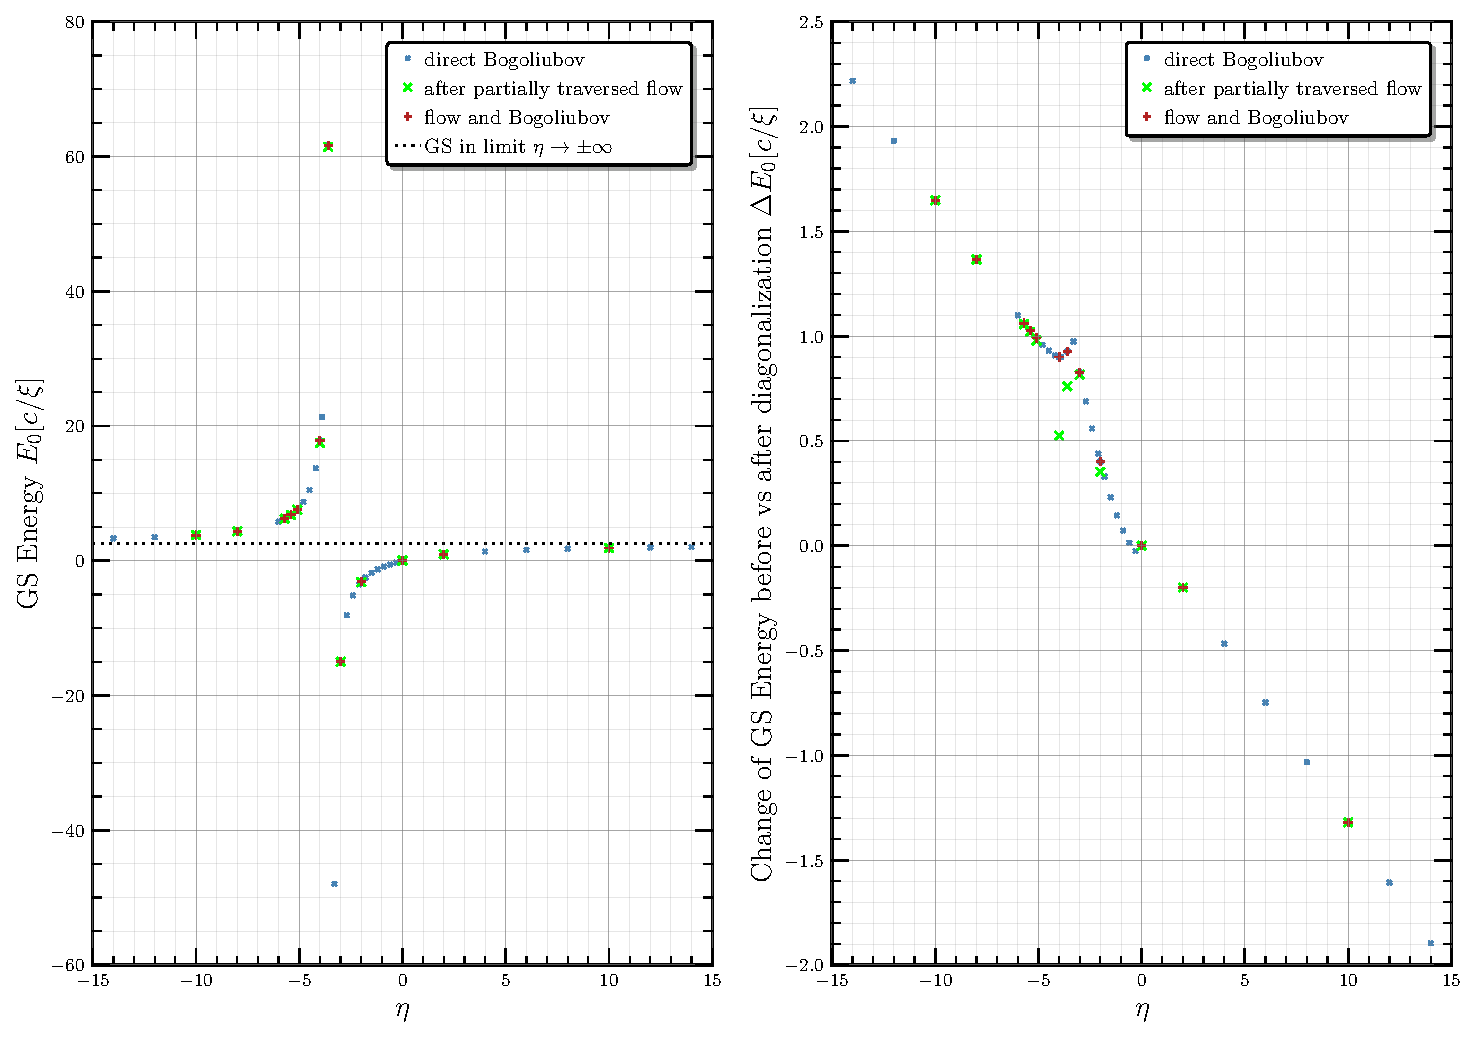
\includegraphics[width=\textwidth]{figures/plots/PDF/GS_energies_bog_flow_comp.pdf}
    \caption[Ground state energy of Bose Polaron for different $\eta$]{The left subplot shows the ground state energy for different $\eta$. The results are obtained via three different approaches: First a Bogoliubov transformation is applied directly to the Hamiltonian \ref{Ham_LLP_qudratic}. Second, the ground state energy is given by the constant $\epsilon$ in the flow Hamiltonian \ref{Flow_Hamiltonian_for_purely_quadratic_case} if all off-diagonal elements are neglected after a sufficiently long traversal of the flow. Third, the off-diagonal elements are not neglected but instead set to zero by a Bogoliubov Transformation of the flow Hamiltonian after traversing the flow for as long as in the second case.
The right subplot shows the difference between the ground state energy and the constant terms in the Hamiltonian \ref{Ham_LLP_qudratic} to highlight the (slight) differences between the three approaches.\\
}
    \label{GSenergiesBogFlow}
\end{figure}
The agreement of the first and third approach in Figure \ref{GSenergiesBogFlow} is not surprising, since the flow equation approach transforms the Hamiltonian in infinitesimal \emph{unitary} steps. The surprisingly good behavior of the second method (standalone flow equations) seems plausible when we consider that $\mathcal O(N^2)$ flows towards the diagonal, where of course the unitarity of the transformation conserves the trace of Hamiltonian (i.e. the sum of its eigenenergies). The number of $V_{k,k^\prime}$ that do not converge to 0 is only $\mathcal O(N)$, and the number of $W_{k,k^\prime}$ that do not converge to 0 is $\mathcal O(1)$. Therefore, assuming that these terms converge to values that are too large and do not diverge, we expect negligible contributions of these terms to the sum of the eigenenergies if a unitary transformation were performed that would actually make these terms vanish. Now, because the ground state energy depends on the sum of the eigenvalues \cite{PracticalTraining}, the prediction for the ground state energy for our system is very accurate. It is noteworthy that the ground state energy in the limit $\eta\rightarrow\pm\infty$ is the same. This is because the two branches are adiabatically connected\cite{Grusdt_2017}.\\
But an accurate prediction of the ground state energy does not necessarily imply that all eigenenergies are predicted accurately too. 
\begin{figure}[H]
    \centering
    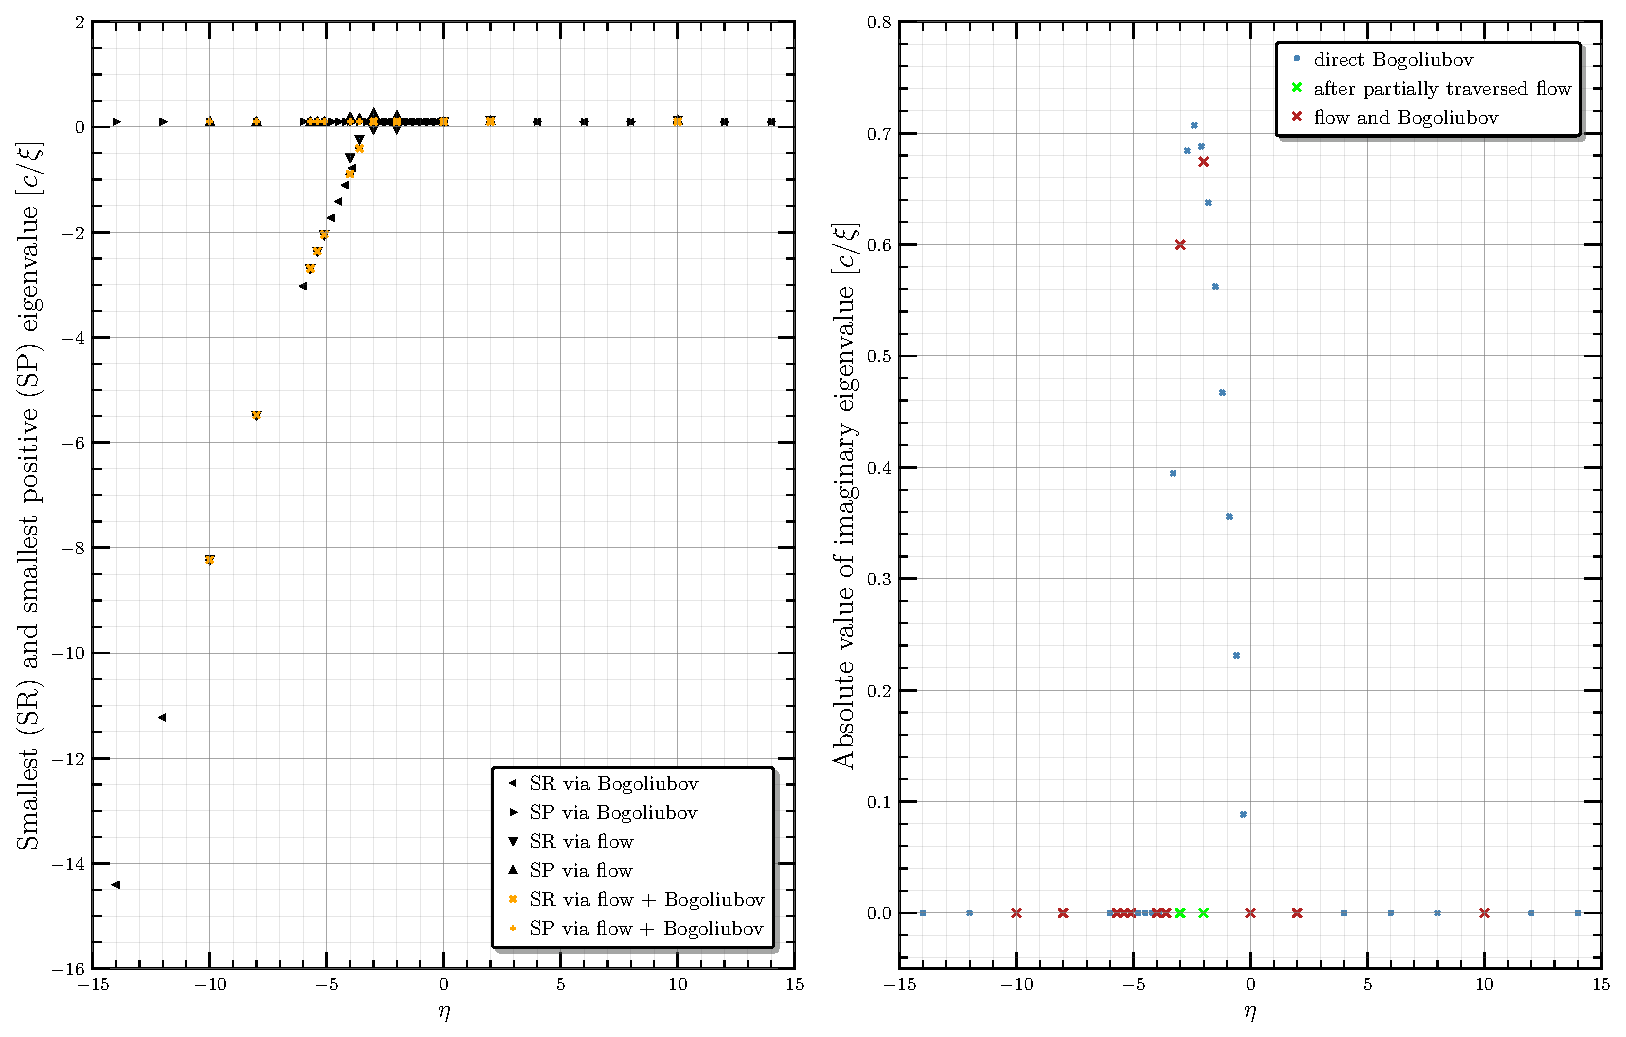
\includegraphics[width=\textwidth]{figures/plots/PDF/spectrum_analysis_bog_flow_comp.pdf}
    \caption[Characteristic eigenenergies of the Bose Polaron for different $\eta$]{The left subplot shows the smallest real (SR) and smallest real positive (SP) eigenvalues of the Hamiltonian for different $\eta$. The right subplot illustrates in which regime dynamical instabilities (i.e. imaginary eigenvalues) occur.
}
    \label{SpectrumAnalysis}
\end{figure}
For example, the difference in the ground state energy in Figure \ref{GSenergiesBogFlow} for $\eta\approx -3.5$, which becomes especially clear when looking at the right subplot, can be explained by the fact that in this regime imaginary eigenvalues are to be expected (see Figure \ref{SpectrumAnalysis}). The flow equations cannot "see" these eigenvalues because the original Hamiltonian is real and the flow equations are algebraically closed in the sense that the flow cannot generate terms from $\C\setminus \R$ if it starts with purely real terms. If the flow equation approach is applied to a Hamiltonian with complex eigenenergies, those will be encoded in behaviour as seen in Figure \ref{FlowIllustrationInsufficient} where not all off-diagonal terms vanish. \\
The thermodynamic instability region for $-3.5\gtrsim\eta$, on the other hand, is correctly predicted in accordance with the results obtained by a Bogoliubov transformation, since negative eigenvalues are generally unproblematic for the flow equations, even though a more complicated convergence behavior may result from these negative eigenvalues, as we observed in Figure \ref{FlowIllustrationInsufficient}.

\subsection{Analysis of the Spectra}
We have seen that the flow equation approach allows for accurate predictions of the ground state energy. The fact that the flow equations simply gloss over the imaginary eigenvalues that can be seen by a Bogoliubov Transformation leads to less good predictions in a small regime around the $\eta$ where the ground state energy diverges. Yet the relative error of these predictions is still small because the absolute error of $\Delta E_0$ in Figure \ref{GSenergiesBogFlow} is bounded whereas the ground energy is not.\\
In the previous section we have also seen that the flow equations predict the negative eigenvalues correctly. Moreover,  Figure \ref{SpectrumAnalysis} showed that the smallest positive real eigenvalue is (almost) constant across the range of $\eta$ we investigated. This is also true for most of the other positive eigenvalues, and only the end of the spectrum shows interesting behavior, so we will take a closer at that.
\begin{figure}[H]
    \centering
    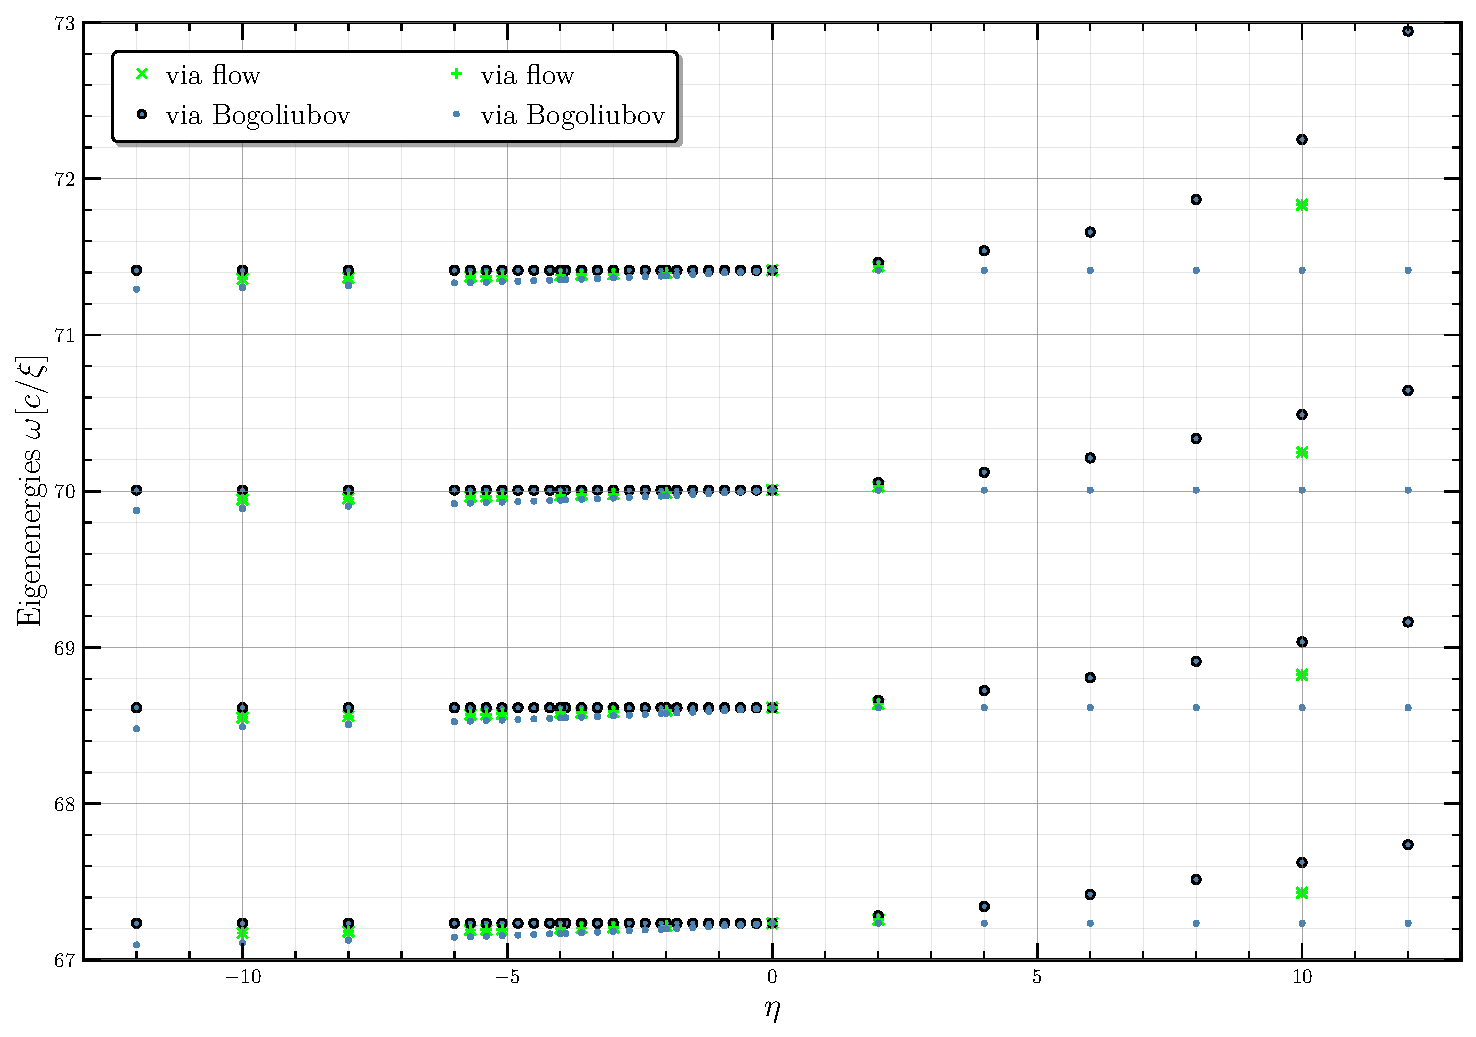
\includegraphics[width=\textwidth]{figures/plots/PDF/SpectralAnalysis.pdf}
    \caption[End of the spectrum of the Hamiltonian for different $\eta$]{This plot shows how the largest eigenvalues change in $\eta$. It has been refrained from performing a Bogoliubov transformation after the flow again, since this would only reproduce the values of a direct Bogoliubov transformation anyway due to the unitarity of the flow transformation.
}
    \label{EndOfSpectrumAnalysis}
\end{figure}
Figure \ref{EndOfSpectrumAnalysis} reveals the following features of the spectrum:
\begin{itemize}
\item The smaller the eigenvalue, the less it changes for different values of $\eta$. This is consistent with the fact, as noted above, that the smallest positive real eigenvalue remains virtually unchanged for different values interaction strengths.
\item In the spectrum we get from the flow equations, each eigenvalue appears exactly twice, i.e. each eigenvalue is twofold degenerate. Therefore the flow does not lift the original degeneracy $\omega_k=\omega_{-k}$.
\item In the spectrum we get from the Bogoliubov transformation, the eigenvalues come in pairs too where one eigenvalue remains exactly constant across different interaction strengths. The other increases strictly monotonically with $\eta$.
\item The eigenvalues from the flow spectrum are almost exactly the mean value between the two different values corresponding to a pair in the Bogoliubov spectrum.
\end{itemize}
If this pattern can be continued, it seems plausible, even without knowing details about the flow equations, that no imaginary eigenvalues can be observed with them: Since the original Hamiltonian is purely real, its characteristic polynomial is also purely real, and its zeros must occur in pairs $\lambda,\lambda^*$. But since $\lambda+\lambda^*\in\R$, the flow equations do not see complex eigenvalues.\\
In the next section, we will try to remove the degeneracy in the flow equations, in the hope that better agreement with the spectrum obtained via the Bogoliubov transformation can be achieved.
%The transformation \ref{twisted_trafo} then follows by again discretizing the momentum space. 
\section{Introducing Twisted Boundary Conditions}
\begin{figure}[H]
    \centering
    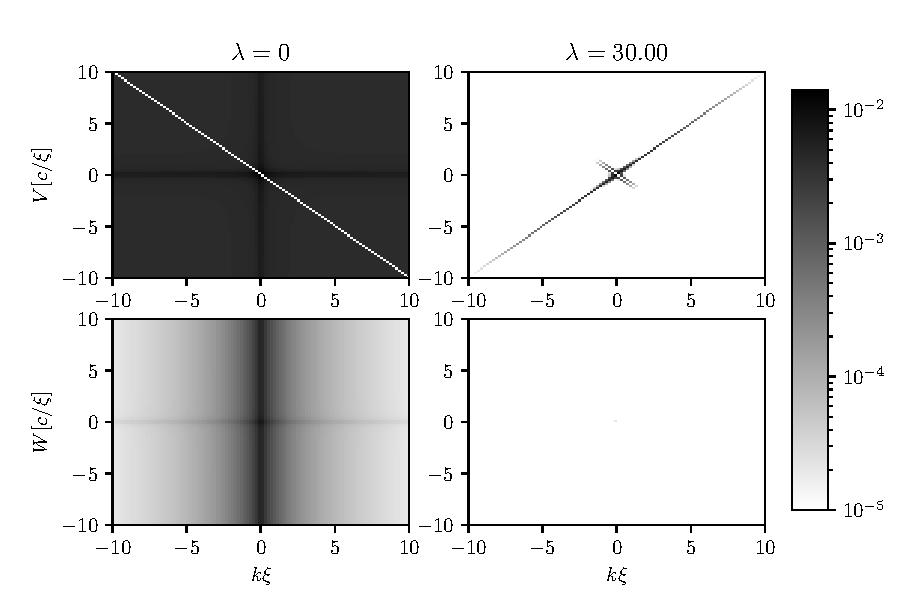
\includegraphics[width=\textwidth]{figures/plots/PDF/FlowIllustrationPhi.pdf}
    \caption[Flow Visualization for $\eta=0.2$ and $\varphi = 1$]{Visualization of the flow progression for $\eta=0.2$ and $\varphi = 1$ analogous to Figure \ref{FlowIllustration}. We can see that by introducing the symmetry breaking parameter $\varphi$, all $V_{k,k^\prime}$ decay from the outside, albeit slowly. Yet, considering the shading scale is logarithmic, many $V_{k,k^\prime}$ can be well suppressed even if the flow is stopped at $\lambda=30$.}
    \label{FlowIllustrationPhi}
\end{figure}
We will now try to improve the convergence properties of the off-diagonal matrix elements using the transformation
\begin{equation} \label{twisted_trafo}
\left\{\Delta k_n\right\}_{n\in\Z}\rightarrow \left\{\Delta k_n+\frac{\varphi}{L}\right\}_{n\in\Z}
\end{equation}
 which (slightly) shifts the grid of $k$-values and thereby breaks the symmetry $k\leftrightarrow -k$ by introducing a phase parameter $\varphi\in\R$. Obviously the original, symmetrical grid is recovered in the limit $\varphi\rightarrow 0$. 
This transformation is not merely a mathematically convenient trick but is also physically meaningful. If we consider our BEC in which the impurity is immersed arranged in circular form we expect periodic boundary conditions
\begin{equation}
\psi(x)=\psi(x+L)
\end{equation}
on a wave function $\psi$ describing some part of the system. However, introducing a magnetic flux $\theta$ in the ring imposes \emph{twisted} periodic boundary conditions:
\begin{equation}
\psi(x)=e^{i\varphi}\psi(x+L)
\end{equation}
It can then be shown \cite{twisted} that these twisted boundary conditions are equivalent to the shift 
\begin{equation}
-i\partial_x\rightarrow -i\partial x+\frac{\varphi}{L}
\end{equation}
or, after recognizing the momentum operator in position representation, 
\begin{equation}
k\rightarrow k+\frac{\varphi}{L}.
\end{equation}
\begin{figure}[H]
    \centering
    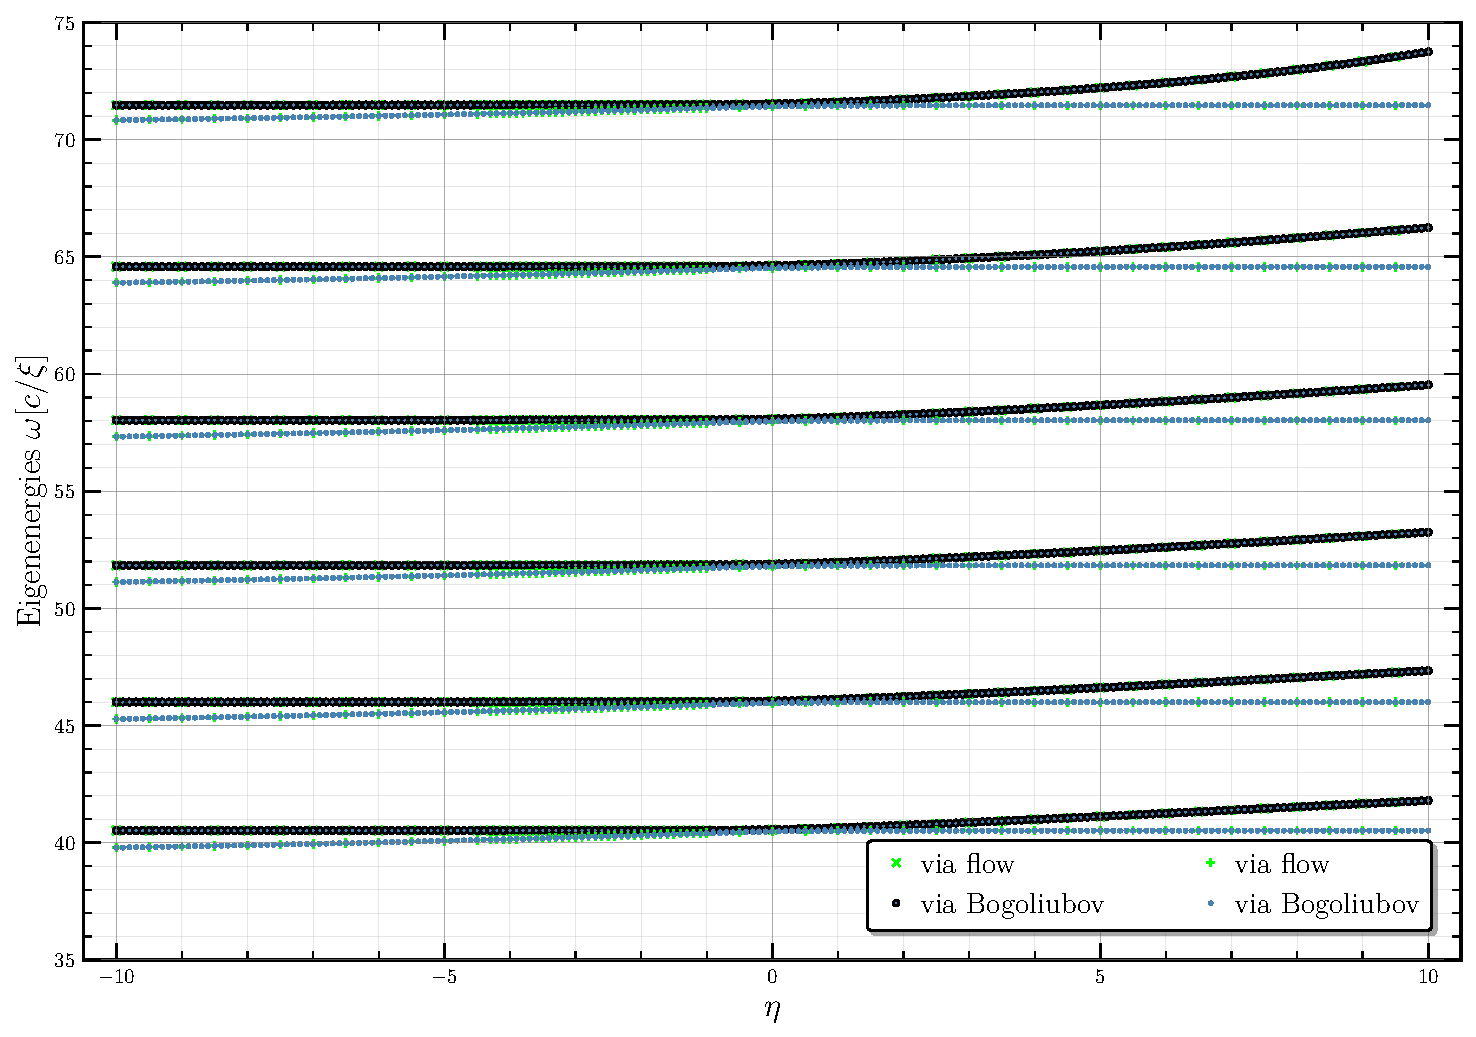
\includegraphics[width=\textwidth]{figures/plots/PDF/Spectral_analysis,N=40.pdf}
    \caption[End of the spectrum of the Hamiltonian with twisted boundary conditions]{This plot shows how the largest eigenvalues change in $\eta$ analogously to Figure \ref{EndOfSpectrumAnalysis} when twisted boundary conditions are in place. We can see that the symmetry breaking helps the convergence of the flow equations to the diagonal Hamiltonian. }
    \label{ConvergenceImprovementsTwisted}
\end{figure}
Indeed, shifting the $k-$grid improves the convergence properties of the $V_{k,k^\prime}$, as seen in Figure \ref{FlowIllustrationPhi}. There the calculations were still based on a $N=200$ grid of $k$-values, just like in the previous section. \\
In the following, we will significantly coarsen the grid to $N=40$ for computational reasons. This is acceptable to get a general idea of the convergence behavior and how the spectrum looks qualitatively, but probably does not allow for quantitatively exact conclusions.
For Figure \ref{ConvergenceImprovementsTwisted} we chose $\varphi\defeq 0.1$. This is a reasonable value because it is large enough to break the symmetry sufficiently much while introducing only a very moderate error of $\sim 1.6\%$ for the smallest $|k|$-value. Hence, the $\omega_k$, $V_{k,k^\prime}$ and $W_{k,k^\prime}$ in the original Hamiltonian have an error of the same order.\\
Since the symmetry of the diagonal part of the original Hamiltonian is now broken, the eigenvalues of the flow Hamiltonian are also no longer degenerate. We obtain a quantitatively very good agreement between the eigenvalues resulting from a Bogoliubov transformation and the predictions of the flow equations for large eigenvalues. Unfortunately, this does not hold for small eigenvalues.
\begin{figure}[H]
    \centering
    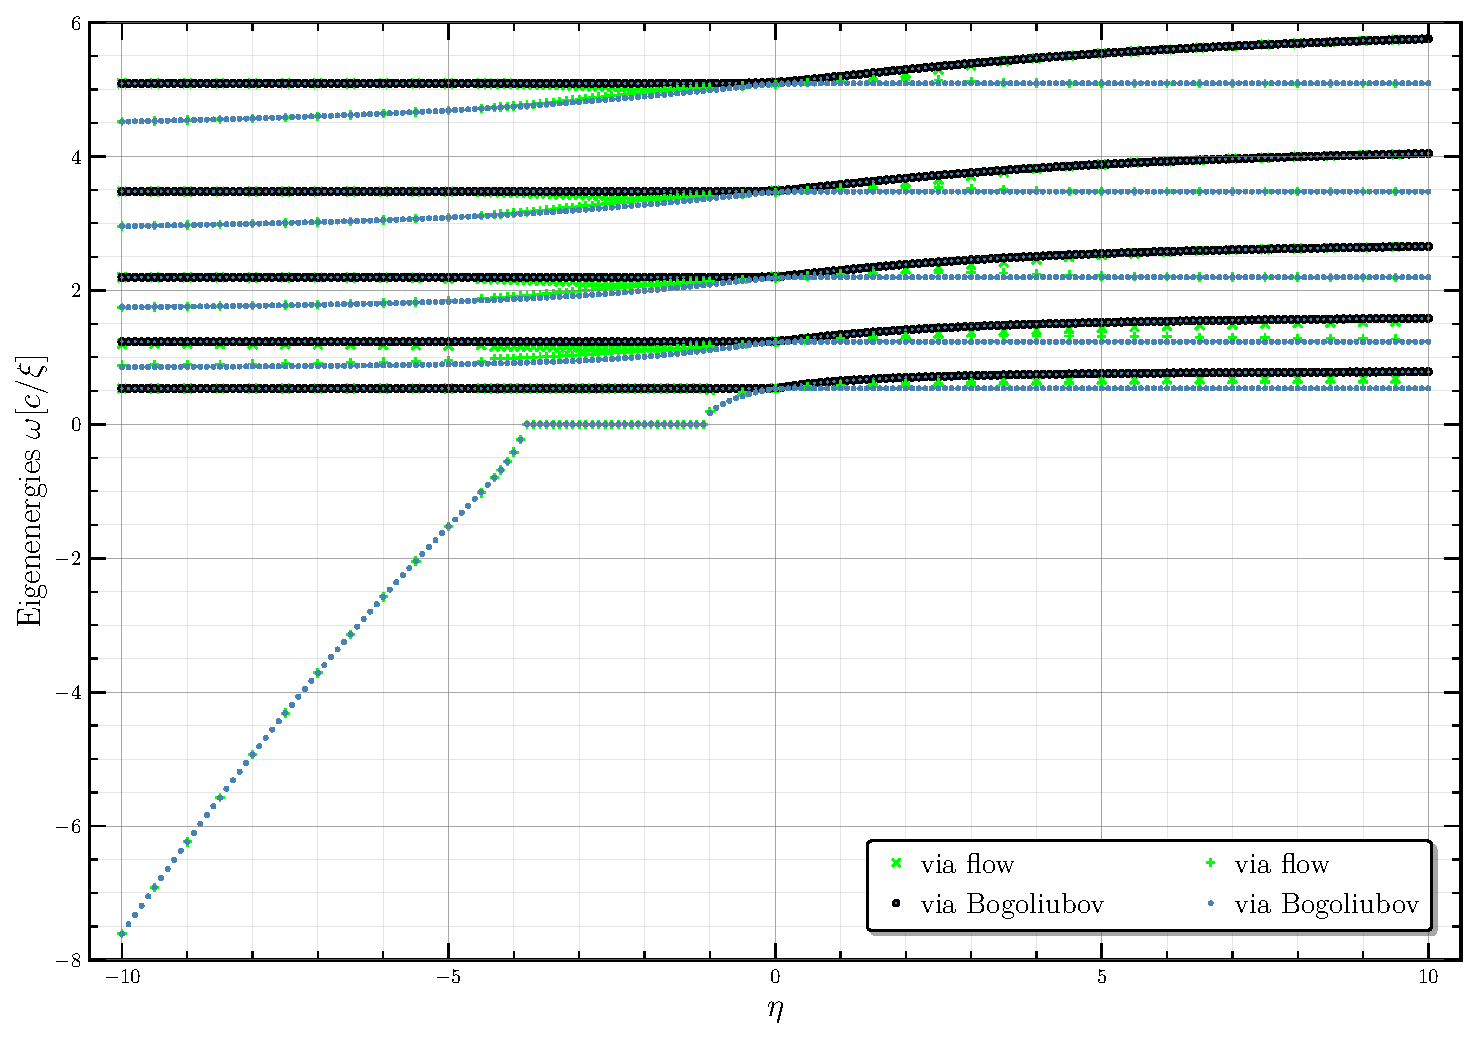
\includegraphics[width=\textwidth]{figures/plots/PDF/Spectral_analysis,N=40_beginning_of_spectrum.pdf}
    \caption[End of the spectrum of the Hamiltonian with twisted boundary conditions]{This plot shows how the smallest eigenvalues change in $\eta$ analogously to Figure \ref{EndOfSpectrumAnalysis} when twisted boundary conditions are in place. We notice a slight discrepancy between the results obtained via Bogoliubov Transformation and via the Flow Equations.}
    \label{ConvergenceTwistedSmallEigenvalues}
\end{figure}
However, it is assumed that these discrepancies can be largely resolved by refining the $k$ grid, since we have very good agreement between the two methods for the top and bottom eigenvalues. Smaller distances between neighboring $k$ values mean, of course, smaller distances between the eigenvalues of the Hamiltonian and thus smaller distances between the eigenvalues we obtain via the flow equations and the Bogoliubov transformation, respectively.



